\documentclass[../main.tex]{subfiles}
\graphicspath{{\subfix{../images/}}}
\begin{document}

\chapter{Introduction}

\section{Purpose}
This is very much difficult to maintain all the data of a course as a hard copy. Any data can be changed, deleted, added at any time. Such as - A new teacher can be assigned for a course, he also can be changed; And so many student are getting admitted every semester. So, IICT WEBSITE is the solution. IICT WEBSITE is a official website based on marking and resulting system of IICT authorized. The main concept of IICT WEBSITE is to devitalized PGD, MIT courses, their students and teachers data maintenance. 

\section{Intended Audience and Reading Suggestions}
This SRS is for developers, project managers, users and testers. Further the discussion will provide all the internal, external, functional and also non-functional informations about IICT WEBSITE.

\section{Project Scope}
IICT WEBSITE creates a space for Director, Teachers, Students and Office Staffs for maintaining particular programs like - PGD, MIT.\@
\newline
After getting admitted to a programs a student has been given a registration number, by using which he/she can inter from-fill-up page. It will take his/her personal informations, admitted fee imformations.He will be added as a student of that particuler programs after completing his/her payment process. After that he/she can select course of the program and then pay the fee for that. Student profile will contain all his personal informations, past results, recent result and notifications.
\newline
Office staff only post result publicly and also notice. But off course with the permission of Director.  
\newline
Directors' main work is to assign teachers to the courses they will take, create teachers profile and approve mark-sheet. He can move a teacher from one course to another. He also can be a teacher and can also can take the courses and perform all the functionality of teacher like- marking papers. He can also directly post notice to the website, teachers and also students.
\newline
Teachers' account are created by director. They (Teachers) entry marks of the students, can view all the marks of the students and change it after submitted it to the director. Every student of that particular course will be under the teacher who is assigned to that course. 
\newline
\begin{figure}
    \centering
    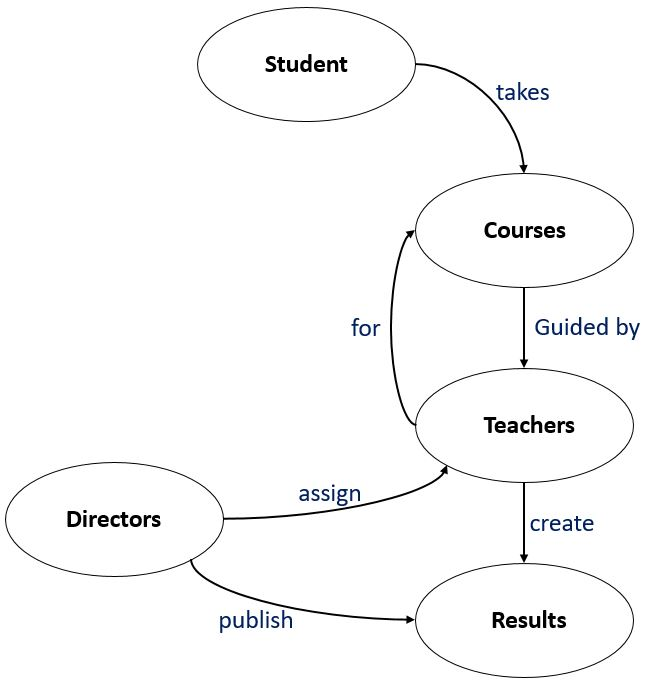
\includegraphics[width=10cm]{../assets/1.JPG}
    \caption{Entire work-flow}
    \label{fig:IICT_WEBSITE}
\end{figure}
\newline
Figure 1.1 (Entire work-flow) is the overview of the project. Connection of all the entities are dependable to each others.  This gives the simple idea about the functional activities of the project. 
\newline
Student cycle, In the Figure 1.1 Student takes Courses; Courses is guided by Teachers; Teachers creates Results. 
\newline
Teacher cycle, In the Figure 1.1 Director assign Teachers; Teachers for particular Courses; Director publish Results.
\newline
So, every entity is vary much interactive with each other.

\end{document}